
\addcontentsline{toc}{section}{Exercițiul 14}
\section*{14. Formulati in limbaj natural si implementati in SQL:}

\vspace{0.5cm}
\begin{enumerate}
    \item \textbf{O cerere ce utilizeaza operatia outerjoin pe minimum 4 tabele.}
    \begin{lstlisting}
/*
Afisati id-ul, numele si email-ul persoanelor care au facut o reclamatie (in primavara) in magazinele care au profitul lunar mai mare de 3000, si a caror chirias este "Jane Smith".

*/

SELECT c.id_client, c.nume_client, c.email
FROM CLIENT c
FULL OUTER JOIN RECLAMATIE r ON c.id_client = r.id_client
FULL OUTER JOIN MAGAZIN m ON r.id_magazin = m.id_magazin
FULL OUTER JOIN CHIRIAS ch ON m.id_chirias = ch.id_chirias
WHERE r.data_ora >= TO_DATE('2023-03-01', 'YYYY-MM-DD') AND r.data_ora < TO_DATE('2023-06-01',
'YYYY-MM-DD')
 AND m.profit_lunar > 3000
 AND ch.nume_chirias = 'Jane Smith';
    \end{lstlisting}
    \vspace{0.2cm}
    \begin{figure}[h]
      \centerline{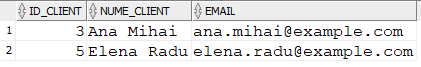
\includegraphics{images/interogare6.png}}
      \caption{ Interogare 6.}
    \end{figure}
    \vspace{0.5cm}

    \item \textbf{O cerere ce utilizează operatia division.}
    \begin{lstlisting}
/*
Afisati toate magazinele care vand doar pantaloni.

*/
SELECT m.nume_magazin
FROM MAGAZIN m
JOIN STOC s ON m.id_magazin = s.id_magazin
JOIN PRODUS p ON s.id_stoc = p.id_stoc
GROUP BY m.id_magazin, m.nume_magazin
HAVING COUNT(DISTINCT p.nume_produs) = 1
AND COUNT(DISTINCT CASE WHEN p.nume_produs = 'Pantaloni' THEN p.nume_produs END) = 1;
    \end{lstlisting}
    \vspace{0.2cm}
    \begin{figure}[h]
      \centerline{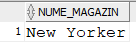
\includegraphics{images/interogare7.png}}
      \caption{ Interogare 7.}
    \end{figure}
    \vspace{0.5cm}

    \item \textbf{O cerere care implementează analiza top-n.}
    \begin{lstlisting}
/*
Top 3 magazine in functie de profit.

*/
SELECT *
FROM (
 SELECT m.id_magazin, m.nume_magazin, m.profit_lunar
 FROM MAGAZIN m
 ORDER BY m.profit_lunar DESC
)
WHERE ROWNUM <= 3;

    \end{lstlisting}
    \vspace{0.2cm}
    \begin{figure}[h]
      \centerline{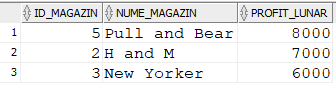
\includegraphics{images/interogare8.png}}
      \caption{ Interogare 8.}
    \end{figure}
\end{enumerate}
